\section{Realisiertes Funktionsmuster}

In diesem Kapitel wird die Umsetzung des in \acrshort{pren1} erarbeiteten Konzept anhand der erstellten Anforderungsliste (siehe Kapitel ``\nameref{anforderungliste}'') bewertet. Der Fokus liegt auf den Fest- und Mindestanforderungen.

\subsection{Anforderungen}

Die physischen Anforderungen an den Roboter konnten vollständig erfüllt werden. Das maximal zulässige Gewicht von 2 kg wurde mit einem Gesamtgewicht von 1.262 kg, insbesondere durch den Einsatz von Leichtbaustrukturen, deutlich unterschritten. Die maximale Baugrösse 300x300x800mm kann in der Startkonfiguration mit Greifer in Ausgangsstellung eingehalten werden. Zusätzlich erforderliche Komponenten wie ein Notausschalter, ein Eingabetaster zur Zieleingabe sowie eine Statusanzeige wurden erfolgreich integriert.

Der Roboter ist in der Lage eine bestimmte Distanz vor und zurück zu fahren und sich einen bestimmten Winkel zu drehen.

Durch diese Funktionen und den Greifer ist der Roboter in der Lage ein Hindernis mit einer Masse von 300g anzuheben und im Umkreis von 20mm am alten Ort abzusetzen. Auf Abbildungen \ref{fig:greifer-open} \& \ref{fig:griefe-rclose} ist das Greifen gezeigt.


\begin{figure}[H]
\centering
\begin{minipage}[b]{0.49\textwidth}
  \centering
    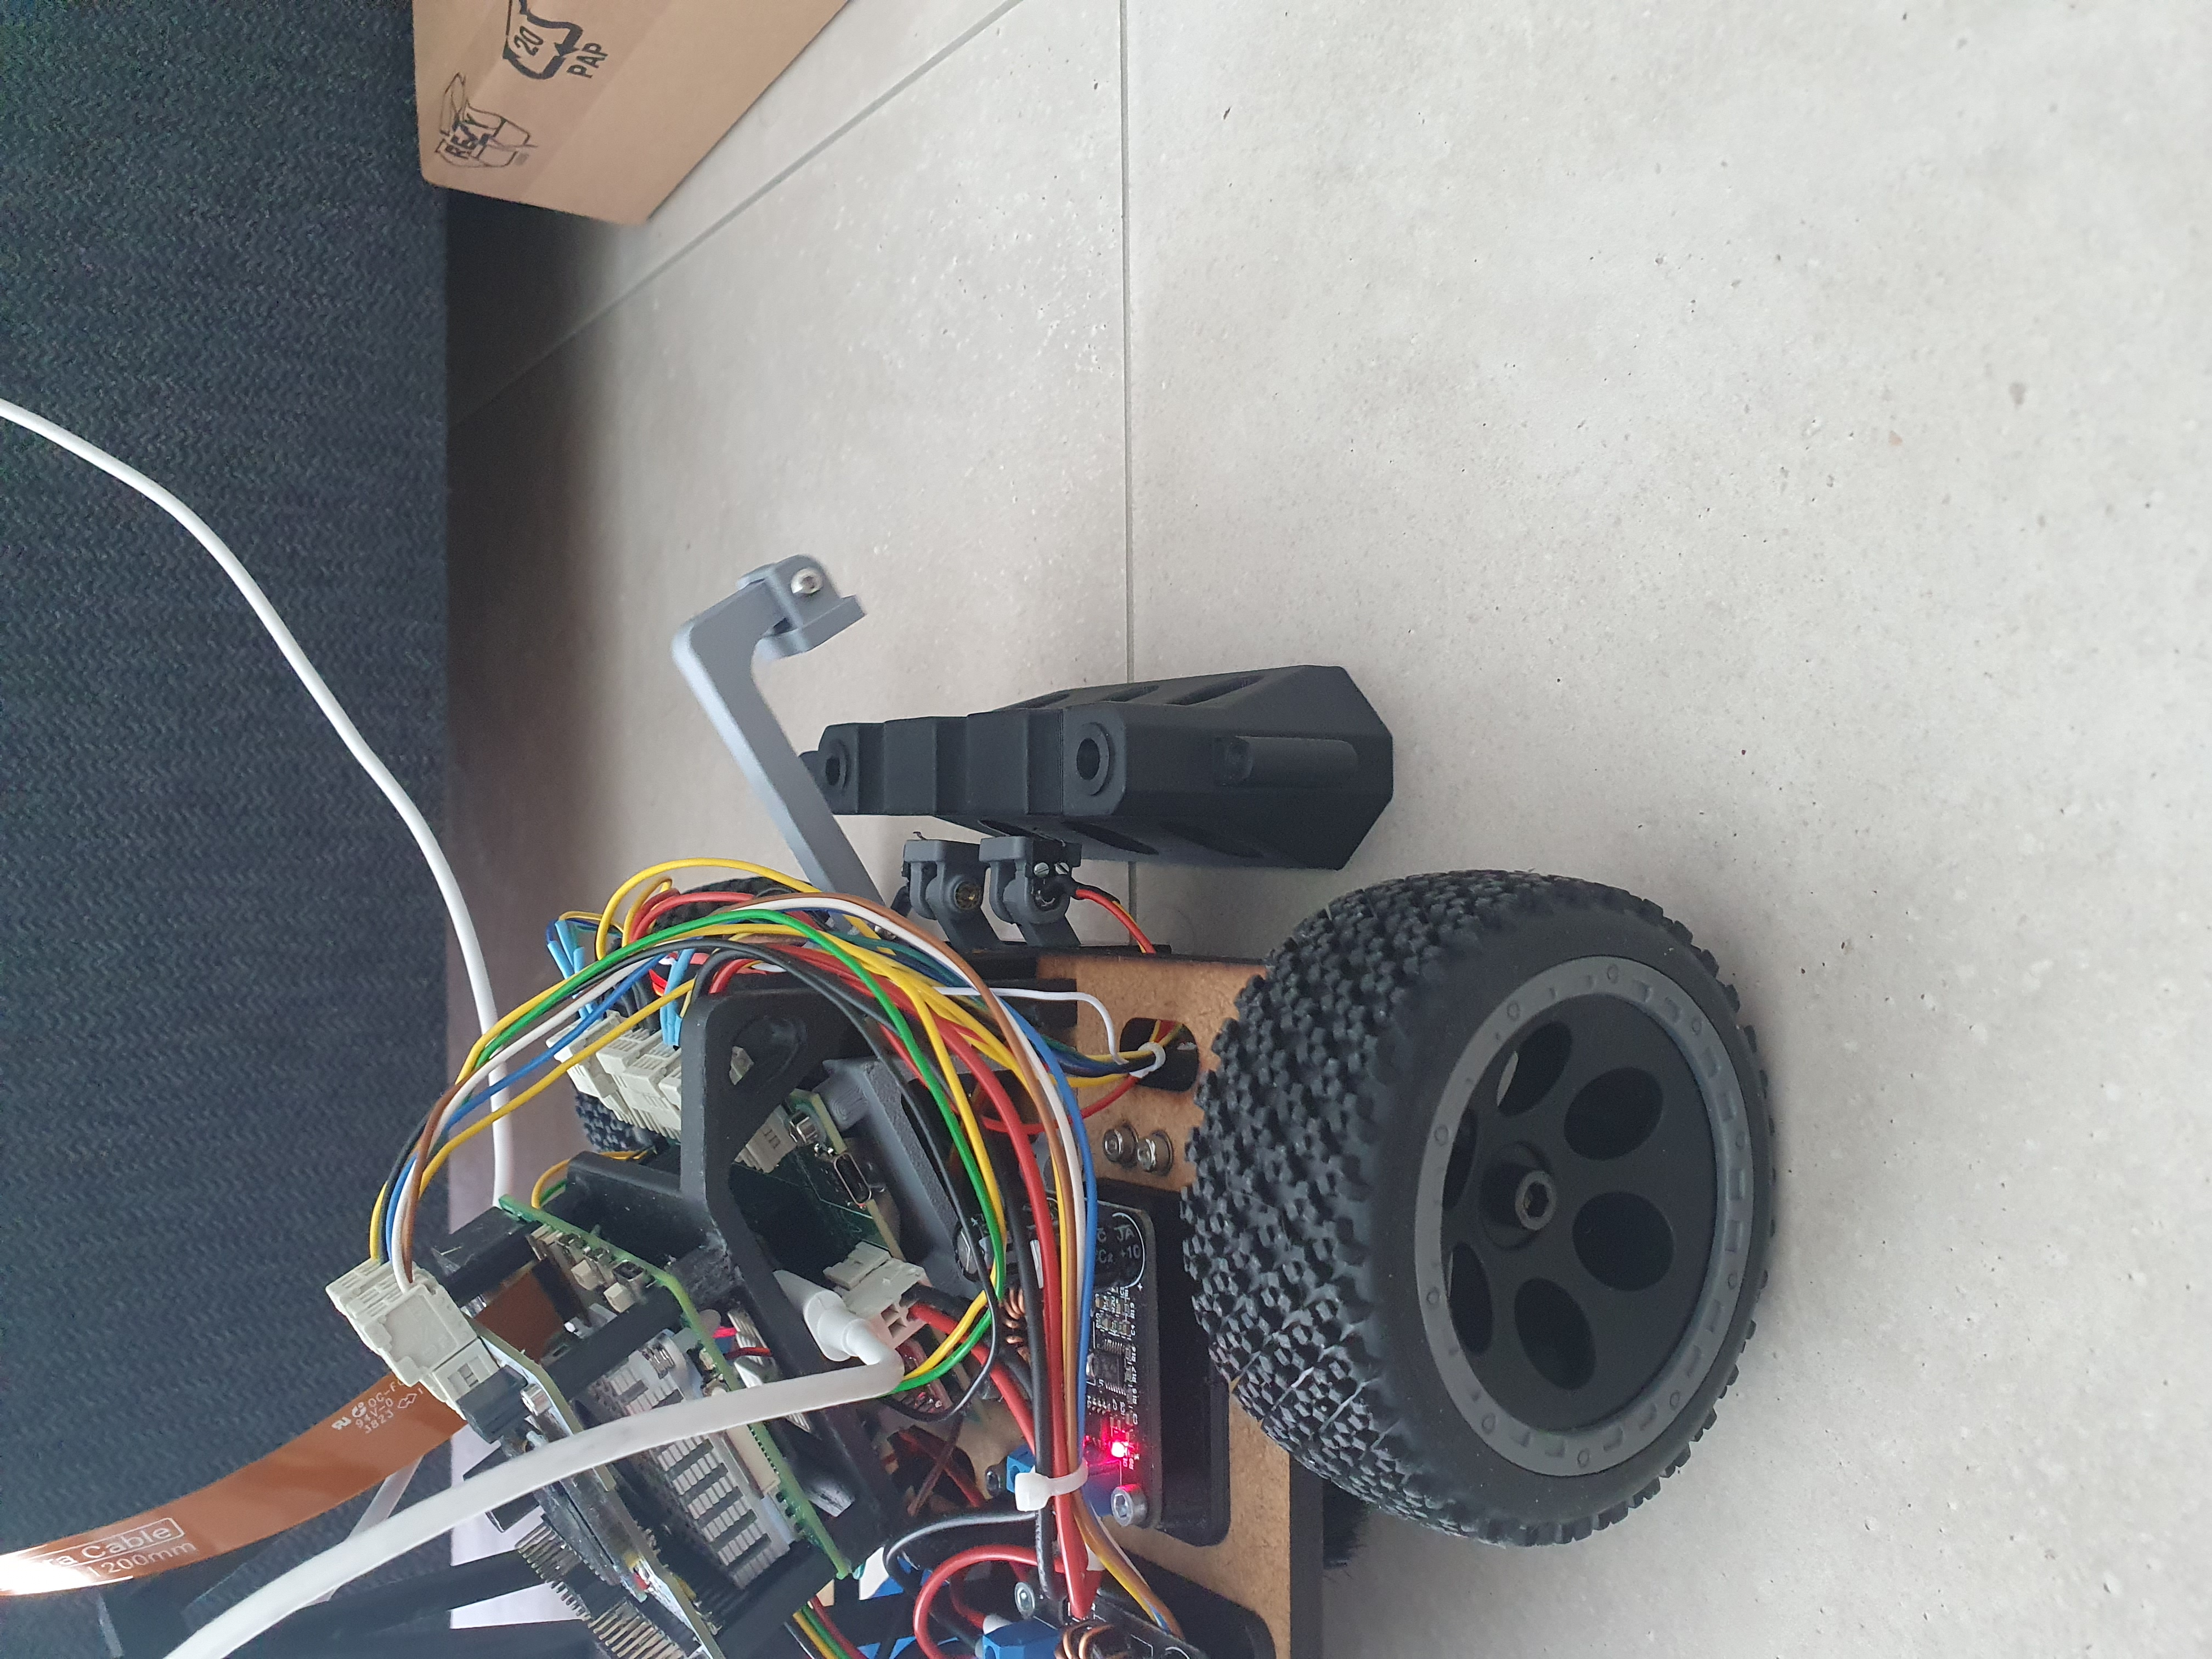
\includegraphics[width=\textwidth, angle=-90]{assets/MT/greifer-open.jpg}
    \caption{Greifer offen}
    \label{fig:greifer-open}
\end{minipage}
\hfill
\begin{minipage}[b]{0.49\textwidth}
  \centering
  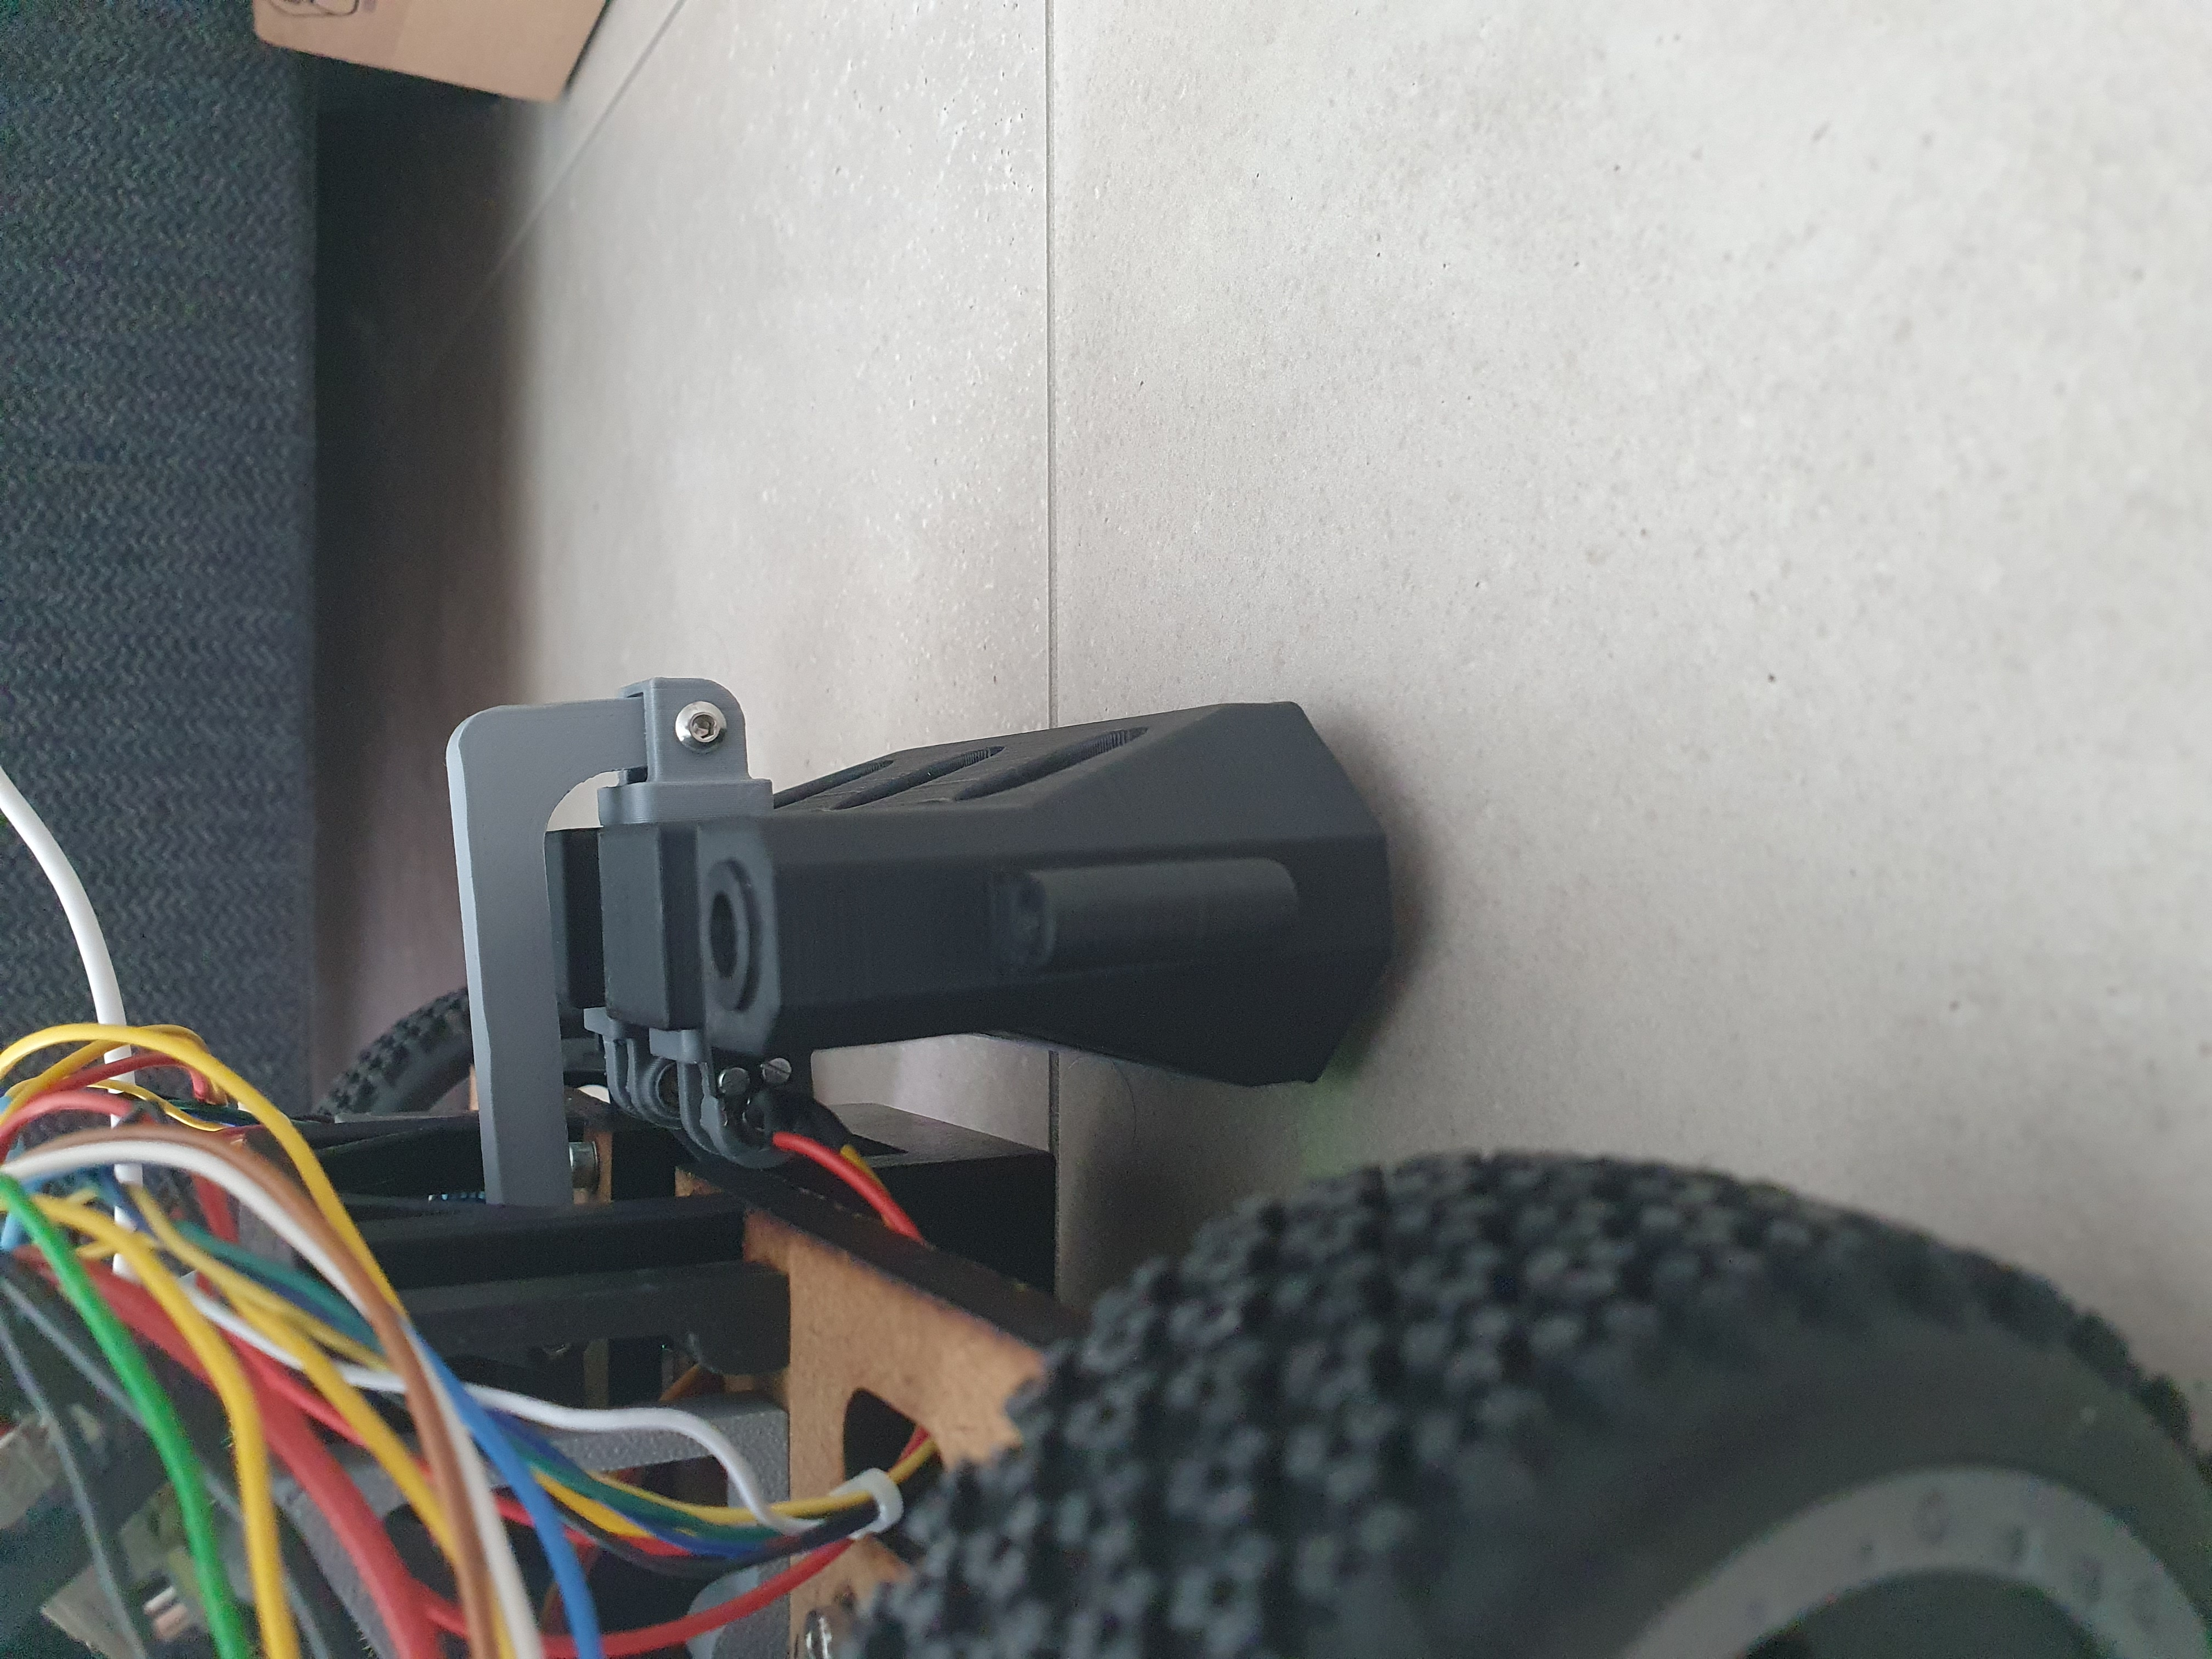
\includegraphics[width=\textwidth, angle=-90]{assets/MT/greifer-close.jpg}
  \caption{Greifer geschlossen}
  \label{fig:griefe-rclose}
\end{minipage}
\end{figure}

Das Folgen der Linie erfolgt wie in \acrshort{pren1} geplant mit einem Liniensensor, der aus mehreren Phototransistoren besteht. Die Regelung der Motoren erfolgt mit Hilfe eines PD-Reglers. Der PD-Regler konnte auf dem Testparcour geprüft werden und ist in der Lage der Linie zu folgen und auf einem Knoten anzuhalten.


% Used hyperlink beceause of includepdf instead of section to label
Die Bilderkennung und der Wegfindungsalgorithmus konnten mithilfe des Kameratestaufbaus aus \acrshort{pren1} und einem leicht veränderten Code bereits vor Ort getestet werden (siehe Anhang \hyperlink{statische-traver.1}{Testprotokoll Statische Traversierung}). Gesperrte Knoten konnten bei den Testläufen mit einer 100\% Sicherheit erkennt werden, ebenso konnten die Barrieren in 100\% der Fälle erkannt werden. Dies bezieht sich auf die manuellen Testdurchläufe und das Trainingsresultat des Models (siehe \gls{confusion-matrix} auf Abbildung \ref{fig:conf-matrix-model}. Trotzdem wird mit dem Ultraschall eine zusätzliche Sicherung eingebaut. Dieser misst auf \pm 1cm zuverlässig, wie nahe sich ein Objekt vor dem Roboter befindet.

Auch die Erkennung der ausgehenden Kanten war immer erfolgreich. Der Algorithmus hat bei allen Testdurchläufen einen direkten Weg ins Ziel gefunden. 

\begin{figure}[H]
\centering
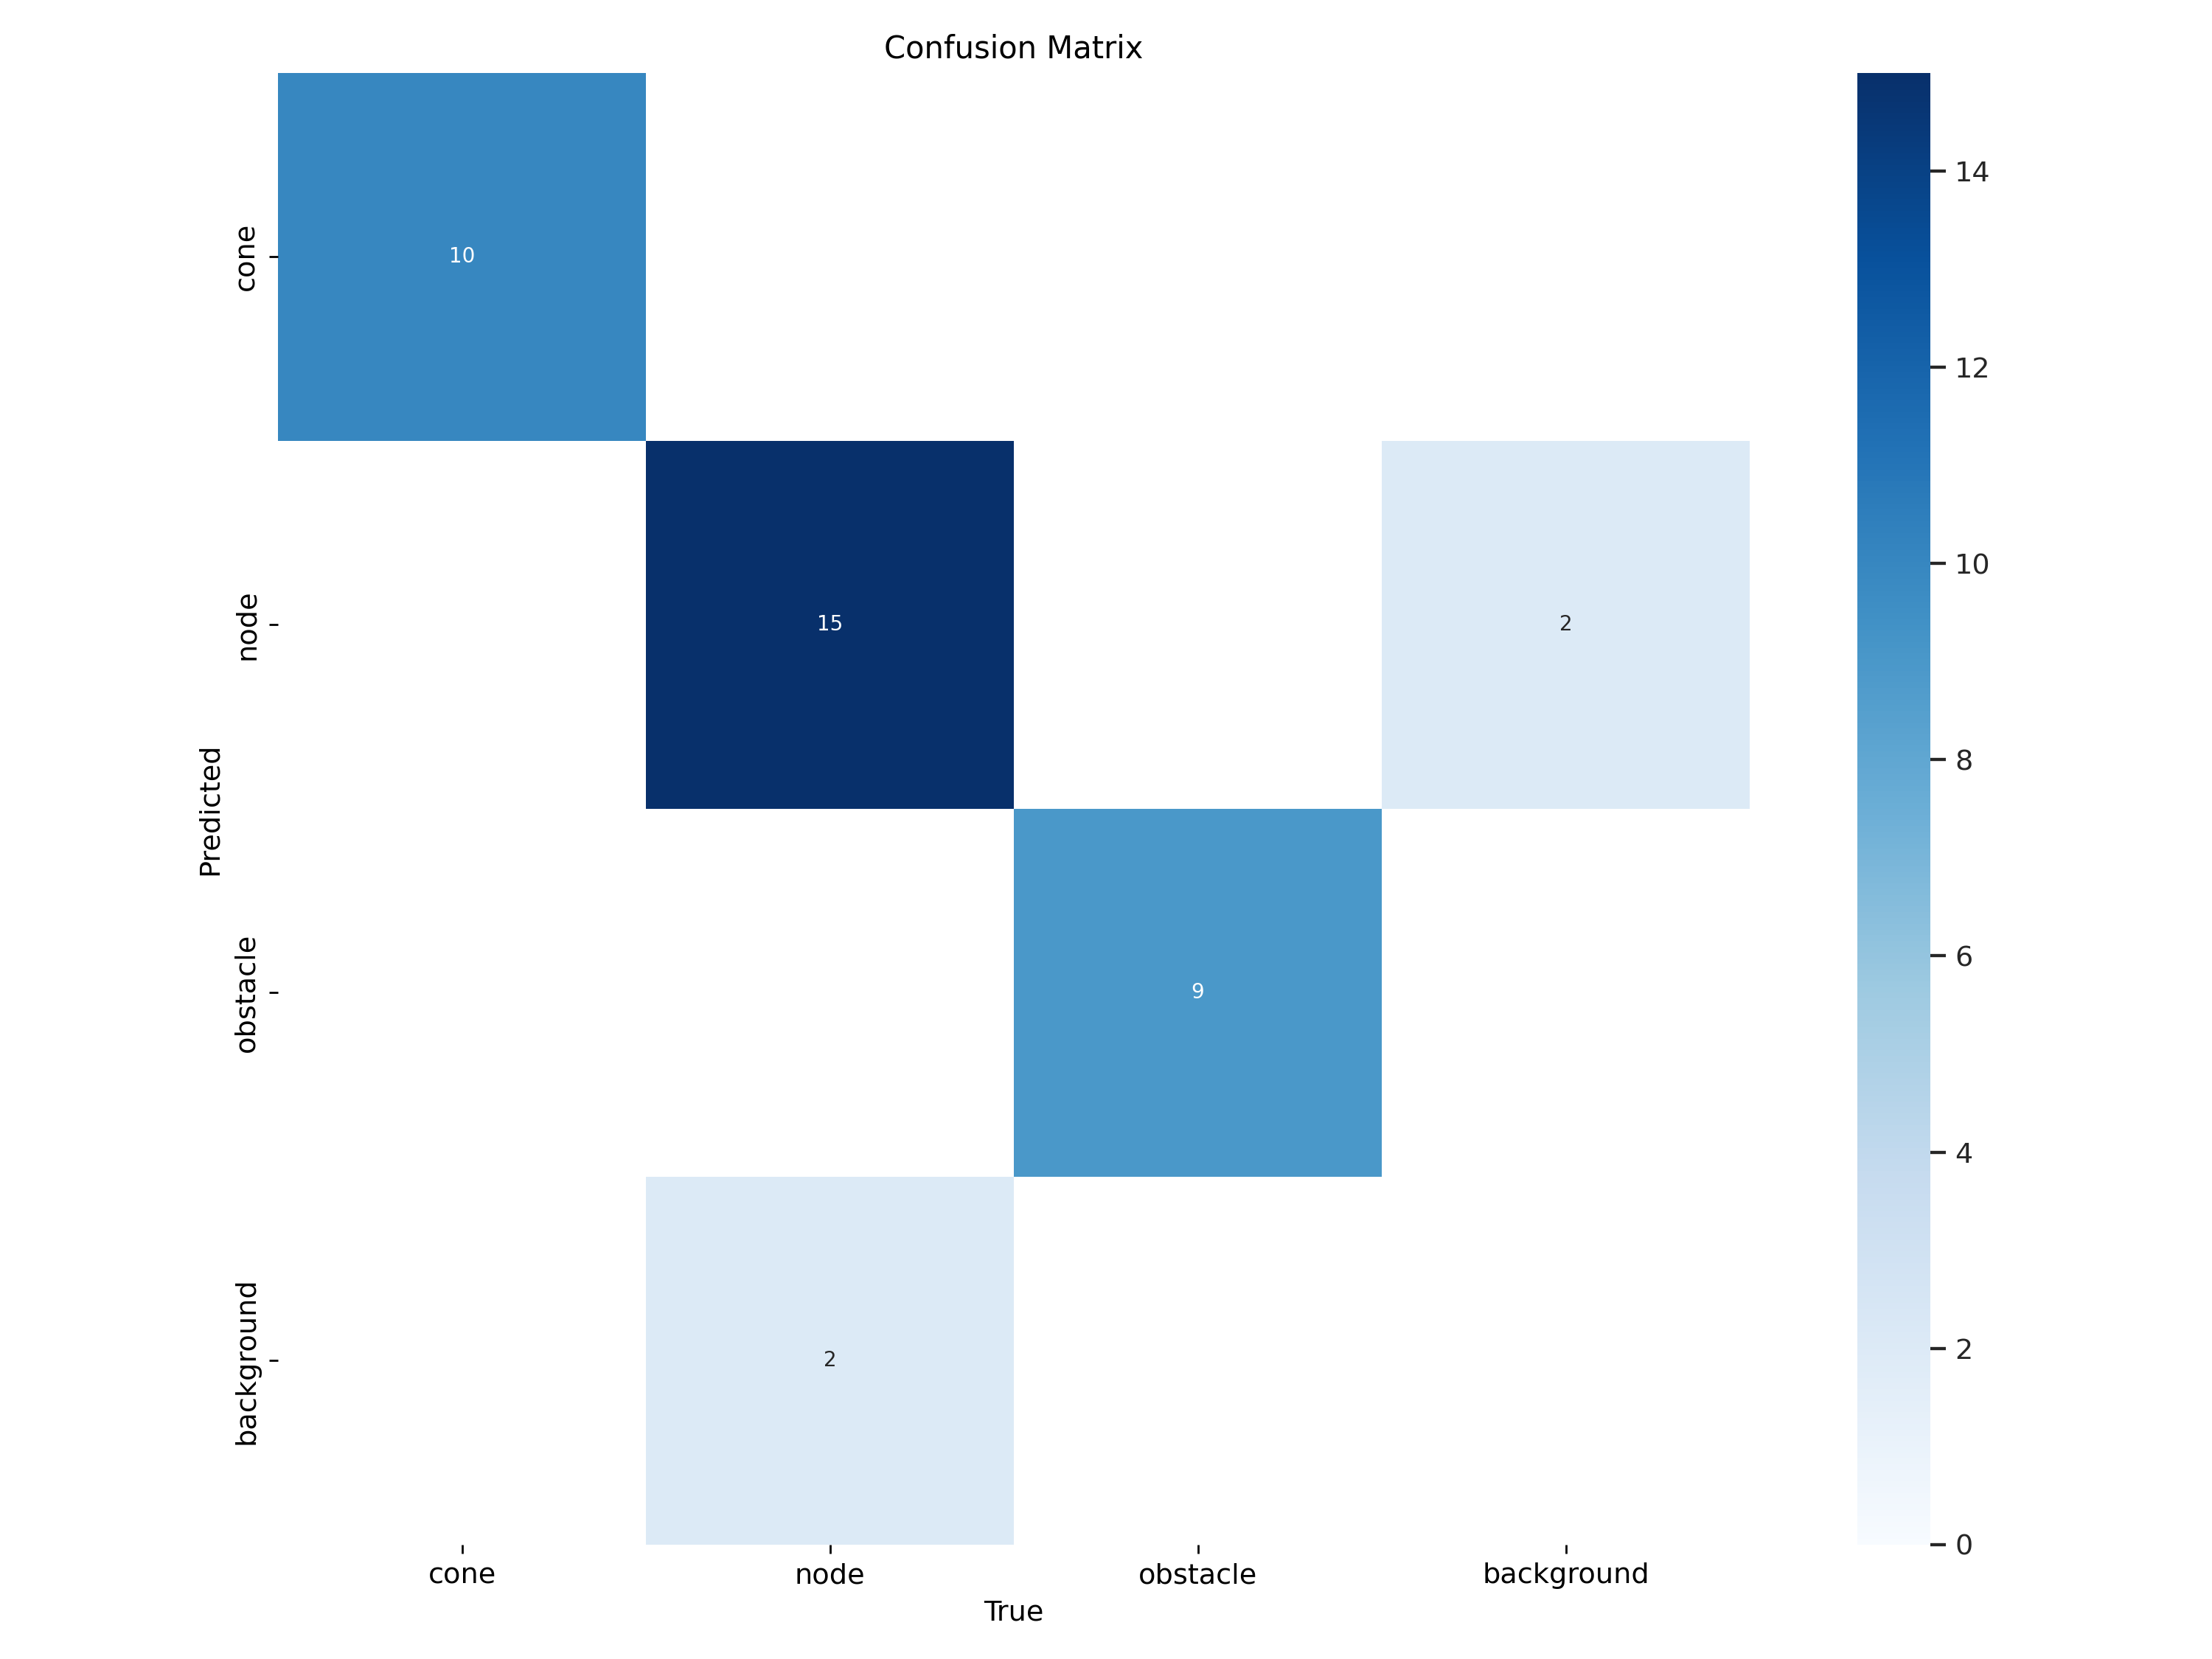
\includegraphics[width=10cm]{assets/IT/yolo/confusion_matrix.png}
\caption{Confusion Matrix Bilderkennung}
\label{fig:conf-matrix-model}
\end{figure}

Es kann ein Ziel ausgewählt werden und der Roboter kann gestartet werden. Die Zielknoten können zuverlässig erkannt werden, was mit realistischen Tests geprüft wurde. Der Buzzersound, der angibt, dass das Ziel erreicht wurde, ertönt schnell und laut.

Der Roboter kann über einen Schalter ein- und ausgeschaltet werden.

Die Konstruktionswerkstoffe konnten wie in PREN1 vorgesehen unter Berücksichtigung der im Kapitel \ref{nachhaltigkeit} Nachhaltigkeit aufgeführten Kriterien ausgewählt werden und fast alle Risiken konnten gemindert werden.

Obwohl fast alle einzelnen Anforderungen erfüllt werden konnten, kann der Roboter momentan nicht das Wegenetz durchqueren. Die Steuerung konnte bis jetzt noch nicht zusammengefügt werden. Die Navigation und die Mechanik funktionieren jedoch beide als Teilsystem.